%!TEX root = spack-paper-sc15.tex

\subsection{The ARES Multi-physics Code}
\label{sec:ares}

\begin{figure*}
	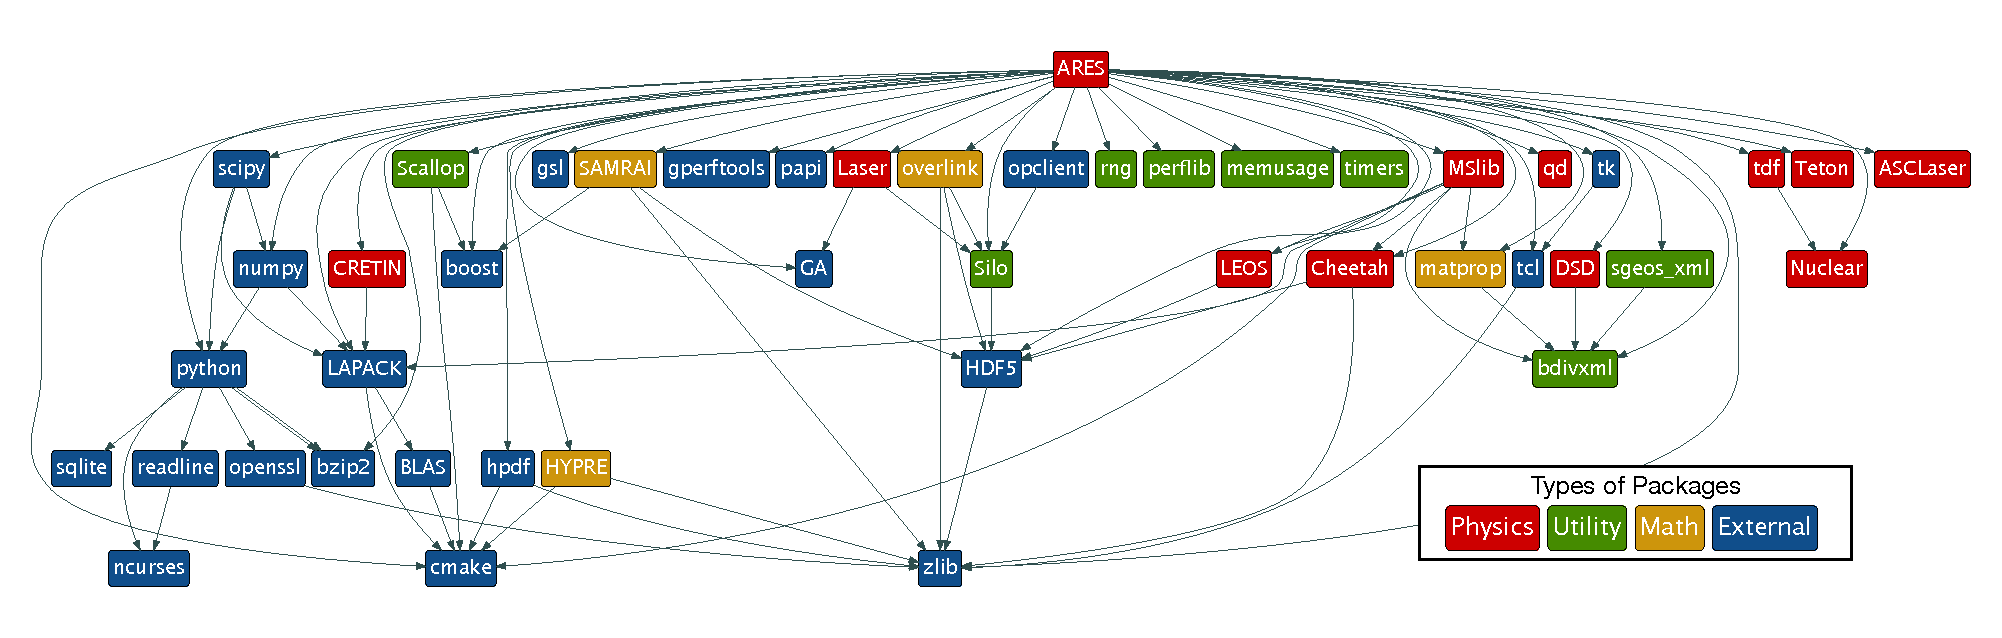
\includegraphics[width=\textwidth]{figs/ares-dot/ares-fig.pdf}
	\caption{
		Dependencies of ARES, colored by type of package.
		\label{fig:ares}
	}
\end{figure*}

\begin{figure}
\begin{tabular}
\end{figure}

For our final use case, we describe our experiences with ARES, a multi-physics code used
in production at LLNL. ARES~\cite{ares1,ares2} is a 1, 2 and 3-dimensional radiation
hydrodynamics code capable of running small serial to large massively parallel simulations.
It is used primarily in munitions modeling and inertial confinement fusion simulations.
%
ARES runs on commodity Linux clusters and on Blue Gene/Q systems at LLNL.  It also
runs on the Cielo Cray XE6 system at Los Alamos National Laboratory (LANL), and it is being
ported to LANL's forthcoming Trinity Cray XC30 machine, using Trinitite, a smaller version
of the full system.  The Trinity machine will consist of two partitions; 
one using Intel Haswell processors and another using Intel Knights Landing processors.
Currently, only the Haswell partition is deployed on Trinitite.

ARES comprises 47 packages, with complex dependency relationships.  The DAG for
the current production configuration of ARES is shown in Figure~\ref{fig:ares}.
At the top is ARES itself.  ARES depends on 11 LLNL physics packages (red), 
4 LLNL math/meshing libraries (gold), and 8 LLNL utility libraries (green).
The utility libraries handle tasks including logging, I/O, and performance
measurement. In addition, ARES uses 23 external software packages, including MPI, BLAS, 
Python, and many other libraries.  Together, these packages ares written in a diverse
set of languages (C, C++, Fortran, Python, tcl) using MPI and OpenMP for parallelism. 
In the configuration we describe here, we have configured Spack to build ARES with
external MPI implementations, depending on the host system. This is a common
configuration, because the vendor- or site-supplied MPI installation is often
optimized and integrated tightly with network drivers on the host system. MPI is shown
as a virtual dependency in the figure, as the implementation differs according to the
host machine.






